\section{Edward O'Brien}\label{per:Edward2OBrien}

\MainPerson{Edward\textsuperscript{2} O'Brien}\index{O'Brien!Edward/Edmund\textsuperscript{2}|bb} aka Edmund\cite{Edmund} (\Lineage{1}{William}) was born in Watergrasshill, County Cork, Ireland,\index{Ireland!Watergrasshill, County Cork} on 10 October 1822.\cite{Edward2OBrienNaturalization} He died in Boston, Suffolk County, Massachusetts,\index{Massachusetts!Boston} on 25 August 1881\cite{Edward2OBrienDeath} and is buried at Holy Cross Cemetery, Malden, Middlesex County, Massachusetts.\cite{CarolGordon}\index{Holy Cross Cemetery}\index{Massachusetts!Malden} He married \MainPerson{Bridget Linne\-han},\index{Linehan/Linnehan!Bridget}\index{O'Brien!Bridget (Linnehan)}\cite{Edward2OBrienMarriage} probably in County Cork, Ireland,\index{Ireland!County Cork} sometime before immigrating to the U.S. on 27 June 1851.\cite{Edward2OBrienNaturalization,Edward2OBrienPetition} Bridget\index{Linehan/Linnehan!Bridget}\index{O'Brien!Bridget (Linnehan)} was born in Ireland\index{Ireland} about 1831\cite{BridgetLinnehanDeath} possibly to William Linnehan\index{Linehan/Linnehan!William} and Jane (\_\_\_\_\_) Linnehan.\index{Linehan/Linnehan!Jane (\_\_\_\_\_)}\index{_@Unknown surnames!Jane}\cite{MaryGrahamDeath} She died in Boston\index{Massachusetts!Boston} on 5 April 1867 of pneumonia\index{pneumonia} at the age of 36.\cite{BridgetLinnehanDeath}

Edward's\index{O'Brien!Edward/Edmund\textsuperscript{2}|bb} profession is listed as ``teamster.''\index{teamster}\cite{LondonStDeed,Edward2OBrien1876} Prior to the use of motorized vehicles, this term referred to a person paid to transport goods by horse-drawn wagon.\cite{Teamster}

Edward\index{O'Brien!Edward/Edmund\textsuperscript{2}|bb} lived at first in Boston's Charlestown\index{Massachusetts!Boston!Charlestown}\cite{MaryAnn3OBrienBirth} and North End\index{Massachusetts!Boston!North End}\cite{Edward3OBrienBirth} neighborhoods. In 1870 he paid \$3,000 for the property at 185 London St.\ in East Boston.\index{Massachusetts!Boston!London St.}\cite{LondonStDeed,LondonStMap} Edward acquired a second East Boston property in 1874, when he purchased 307 Havre St.\index{Massachusetts!Boston!Havre St.} for \$3,325 at public auction.\cite{HavrePurchase,HavreMap} Both properties were passed onto Edward's heirs upon his death, although the combined value was reduced to \$3,700 at the time.\cite{Edward2OBrienProbate} His heirs still held title to the properties until at least 1922,\cite{Bromley1922} when the 185 London St.\index{Massachusetts!Boston!London St.} property was being rented out as apartments.\cite{GlobeRobbery} Edward's niece, Frances Elizabeth\textsuperscript{3} (O'Brien) Wickens,\index{Wickens!Frances Elizabeth\textsuperscript{3} (O'Brien)}\index{O'Brien!Frances Elizabeth\textsuperscript{3}} lived there for a time.\cite{Frances3OBrien1914} Edward's daughters, Annie M.\index{O'Brien!Ann Maria\textsuperscript{3}} and Margaret,\index{O'Brien!Margaret A.\textsuperscript{3} (1859--1933)} continued to live at the house on 307 Havre Street\index{Massachusetts!Boston!Havre St.} up until their deaths in the 1930s.\cite{AnnMaria3OBrienDeath,Margaret3OBrienDeath} The properties were likely important sources of wealth for multiple generations of the O'Brien family.\index{O'Brien!family}

\begin{figure}
	\centering
	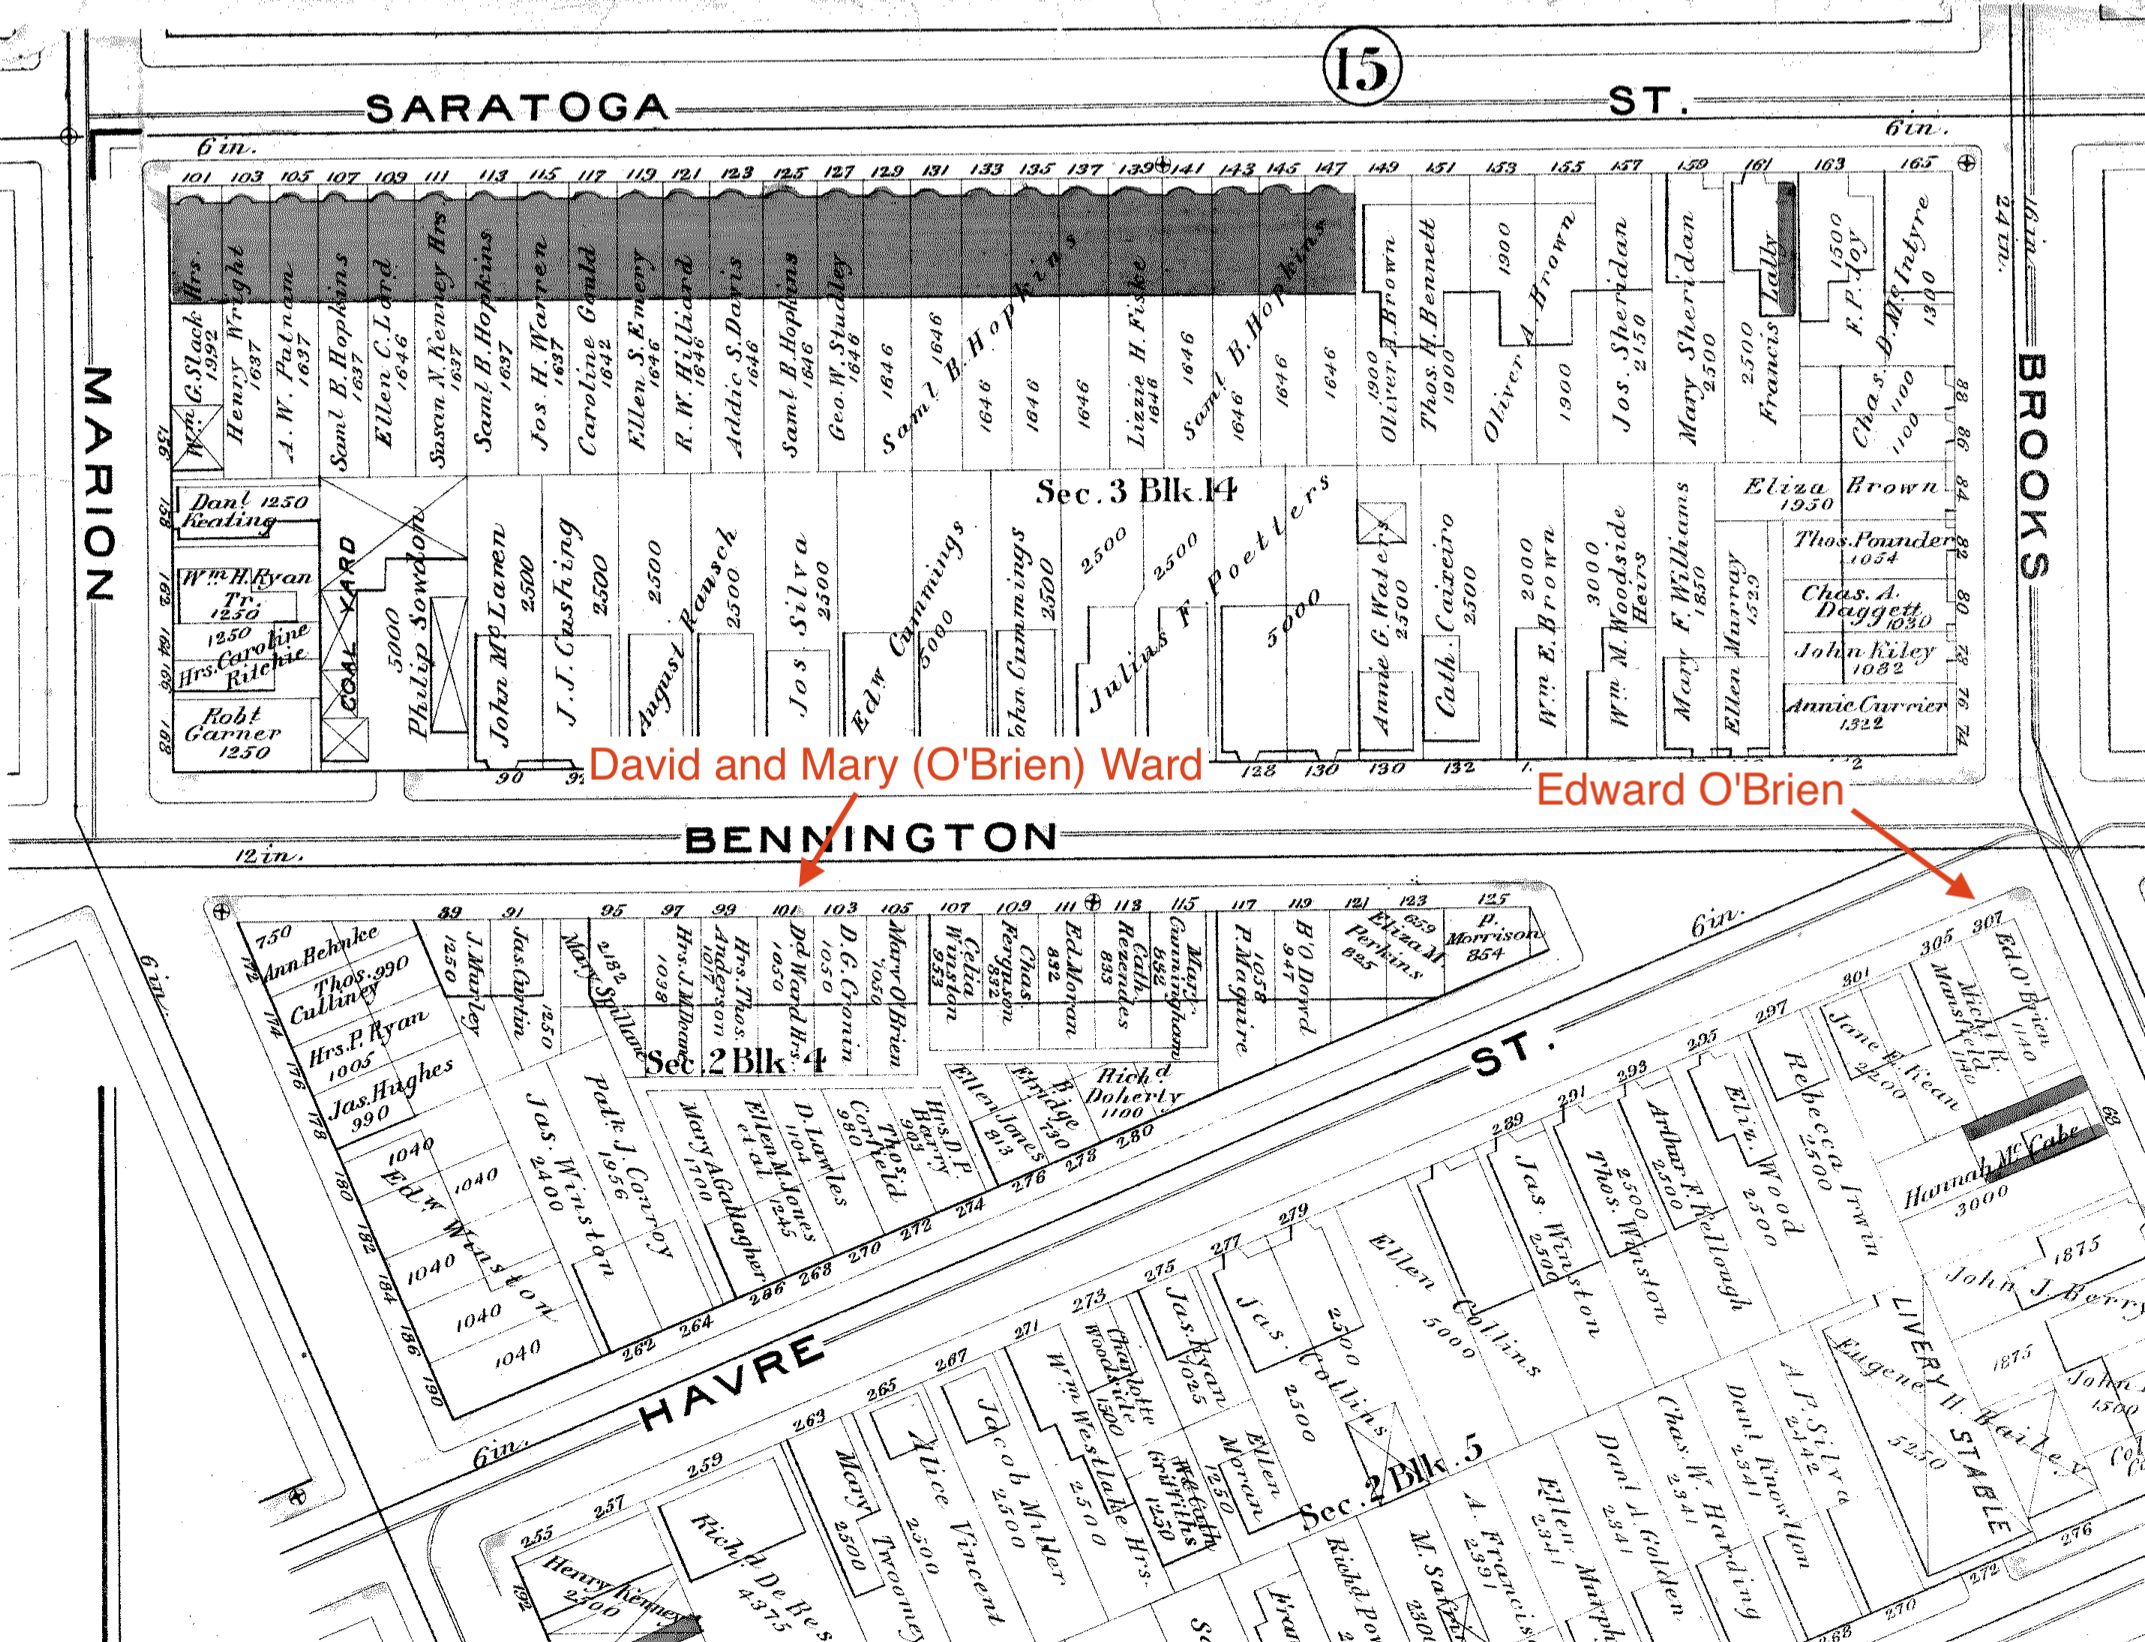
\includegraphics[width=\textwidth]{east_boston}
	\caption{East Boston\index{Massachusetts!Boston!East Boston} map showing the location of Edward O'Brien's\index{O'Brien!Edward/Edmund\string\textsuperscript{2}|bb} and David Ward's\index{Ward!David (husband of Mary (O'Brien))} properties.}
	\label{fig:EastBostonMap}
\end{figure}

Living with Edward\index{O'Brien!Edward/Edmund\textsuperscript{2}|bb} in 1880 were his adult children Annie,\index{O'Brien!Ann Maria\textsuperscript{3}} Margaret,\index{O'Brien!Margaret A.\textsuperscript{3} (1859--1933)} and Edward J.,\index{O'Brien!Edward\textsuperscript{3} (1861--1884)} his sister Ann\textsuperscript{2} (O'Brien) Dailey,\index{Dailey!Ann\textsuperscript{2} (O'Brien)}\index{O'Brien!Ann\textsuperscript{2}} and niece Delia J.,\index{Graham!Delia Jane} age 11.\cite{Census1880Edward} Delia is probably Delia Jane Graham, daughter of William Graham\index{Graham!William} and Mary A (Linehan) Graham.\index{Linehan/Linnehan!Mary A.}\index{Graham!Mary A.\ (Linehan)}\cite{DeliaGrahamBirth,MaryGrahamDeath}\index{Graham!Mary (Linnehan)}\index{Linehan/Linnehan!Mary} Mary could be Bridget's\index{Linehan/Linnehan!Bridget}\index{O'Brien!Bridget (Linnehan)} sister. Edward's household also included Michael Malanny,\index{Malanny!Michael} age 65, and his wife Ann,\index{Malanny!Ann (\_\_\_\_\_)}\index{_@Unknown surnames!Ann} age 62, although their connection to Edward is not known.\cite{Census1880Edward} None of Edward's children ever married. 

There is a large monument at Holy Cross Cemetery\index{Holy Cross Cemetery}\index{Massachusetts!Malden} in Malden marking where Edward is buried along with his wife Bridget, sister Ann, three of his children, and several extended family members. The plot is located at North Monument Ave., Path 17, Grave 34 East (see map in the appendix).\cite{Edward2OBrienGrave,CarolGordon}

\begin{KidsIntro}
	Children of Edward\textsuperscript{2}\index{O'Brien!Edward/Edmund\textsuperscript{2}|bb} and Bridget (Linnehan) O'Brien,\index{Linehan/Linnehan!Bridget}\index{O'Brien!Bridget (Linnehan)} all born in Boston:\index{Massachusetts!Boston}
\end{KidsIntro}

\begin{Kids}
	\KidNum{}{i.}\KidName{Mary Ann\textsuperscript{3} O'Brien},\index{O'Brien!Mary Ann\textsuperscript{3} (1852--1852)} b.\ 13 Oct.\ 1852;\cite{MaryAnn3OBrienBirth} bap.\ Holy Cross (Boston)\index{Holy Cross (church)} 16 Oct.\ 1852;\cite{MaryAnn3OBrienBaptism} d.\ 25 Nov.\ 1852;\cite{MaryAnn3OBrienDeath} bur.\ North Cambridge Catholic Cemetery,\index{North Cambridge Catholic Cemetery}\index{Massachusetts!Cambridge} Cambridge, Middlesex County, Mass.\cite{DianaBerberenaLetter1}
	
	\KidNum{}{ii.}\KidName{Ellen O'Brien},\index{O'Brien!Ellen\textsuperscript{3} (1853--1857)} b.\ 27 Nov.\ 1853;\cite{Ellen3OBrienBirth} bap.\ Holy Cross\index{Holy Cross (church)} 3 Dec.\ 1853;\cite{Ellen3OBrienBaptism} d.\ 10 March 1857;\cite{Ellen3OBrienDeath} bur.\ North Cambridge Catholic Cemetery.\cite{DianaBerberenaLetter2}\index{North Cambridge Catholic Cemetery}
	
	\KidNum{}{iii.}\KidName{Ann Maria ``Annie'' O'Brien},\index{O'Brien!Ann\textsuperscript{3}} b.\ 9 Nov.\ 1855;\cite{AnnMaria3OBrienBirth} bap.\ St.\ John the Baptist (Boston)\index{St.\ John the Baptist (church)} 17 Nov.\ 1855\cite{AnnMaria3OBrienBaptism}; d.\ 24 May 1937;\cite{AnnMaria3OBrienDeath} bur.\ Holy Cross Cemetery.\cite{CarolGordon}\index{Holy Cross Cemetery}
	
	\KidNum{}{iv.}\KidName{Margaret A.\ ``Maggie'' O'Brien},\index{O'Brien!Margaret A.\textsuperscript{3} (1859--1933)} b.\ 22 Aug.\ 1859;\cite{Margaret3OBrienBaptism} bap.\ 29 Aug.\ 1859;\cite{Margaret3OBrienBaptism} d.\ 6 March 1933;\cite{Margaret3OBrienDeath} bur.\ Holy Cross Cemetery.\cite{CarolGordon}\index{Holy Cross Cemetery}
	
	\KidNum{}{v.}\KidName{Edward J.\ O'Brien},\index{O'Brien!Edward\textsuperscript{3} (1861--1884)} b.\ 7 April 1861;\cite{Edward3OBrienBirth} d.\ 7 Jan.\ 1884;\cite{Edward3OBrienDeath} bur.\ Holy Cross Cemetery.\cite{CarolGordon}\index{Holy Cross Cemetery}
\end{Kids}